In this chapter we present the results of our chunking and analysis
methodology on two problems. The first problem is the multiple disk clutch
brake design problem, a discreet optimization problem with five variables
and two objectives. The other is the welded beam design problem which is
continuous decision space problem with four variables and two objectives.

\section{Problem Introduction}
\subsection{Multiple-disk clutch brake design problem}


\begin{figure}[ht]\begin{center}
 \fbox{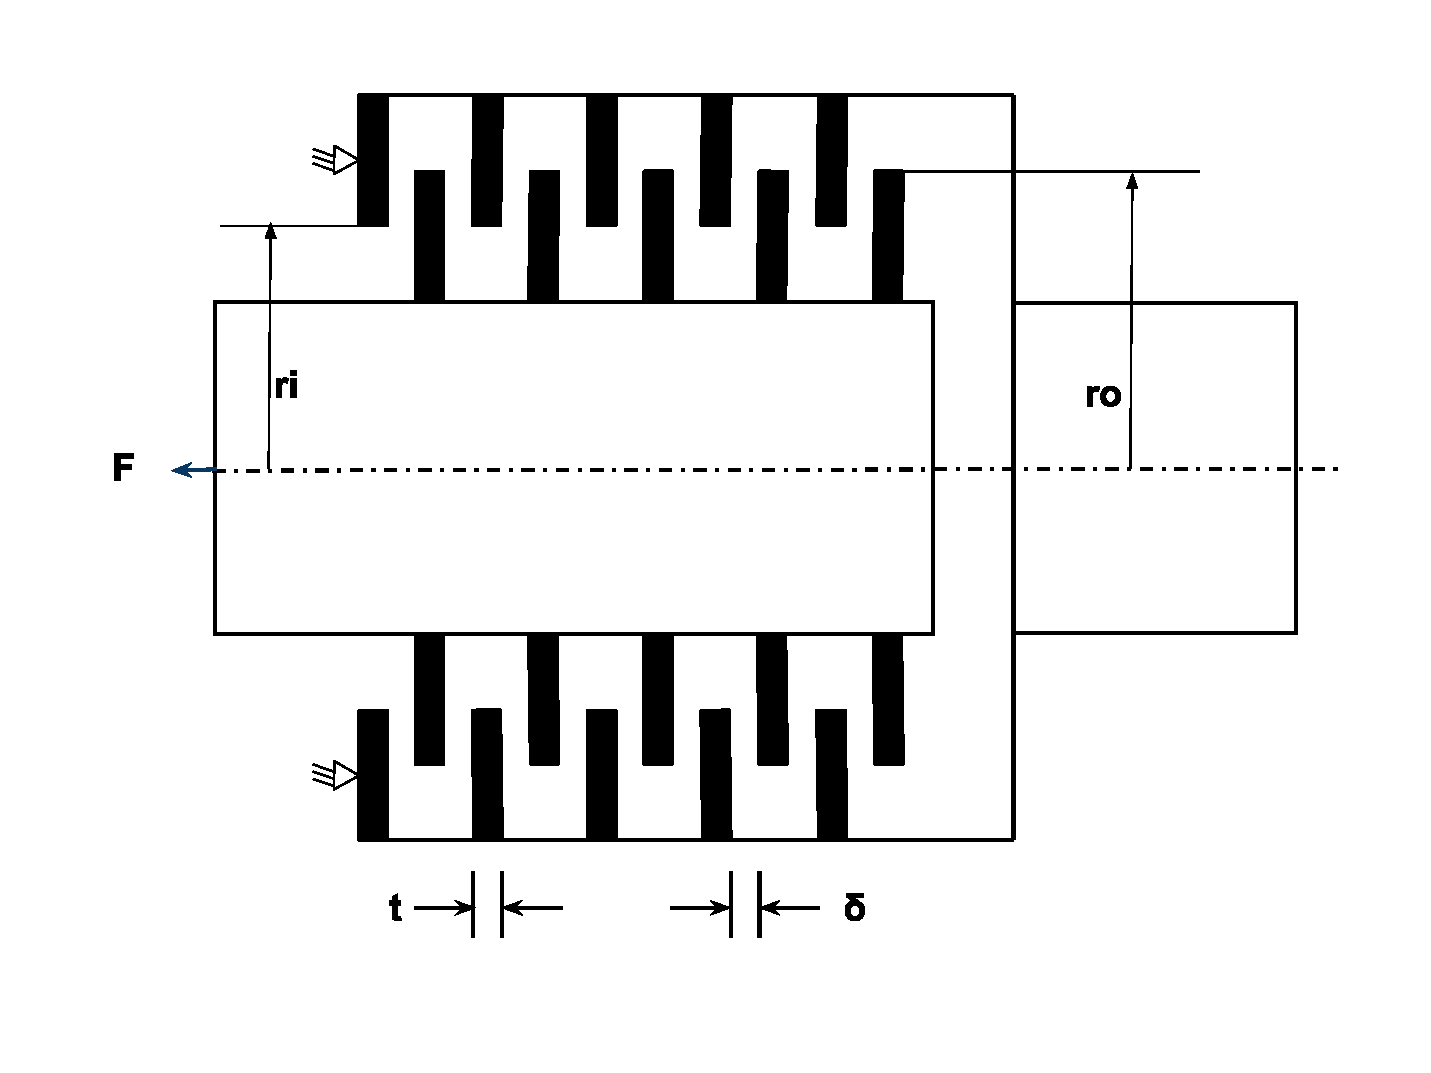
\includegraphics[width=75mm, height=60mm]{dia/clutchbrake.eps}}
 \caption{Schematics of a multiple disk clutch brake.}
 \label{clutchbrake}
\end{center}\end{figure}


We have adopted the problem specification used in \citep{deb06}. The
schematics of a multiple-disk clutch brake are shown in figure
\ref{clutchbrake}. Two conflicting objectives are considered in this 
optimization problem:
{\allowdisplaybreaks \begin{enumerate}
  \item minimization of mass, and,
  \item minimization of stopping time.
\end{enumerate}
This optimization problem is defined on five decision variables $\vec{x} = (r_i, r_o, t, F, Z)$, where:
\begin{enumerate}
  \item $r_i \in [60, 80]$ (in steps of one) is the inner radius in mm,
  \item $r_o \in [91, 110]$ (in steps of one) is the outer radius in mm,
  \item $t \in [1, 3]$ (in steps of 0.5) is the thickness of disks in mm,
  \item $F \in [600, 1000]$ (in steps of 10) is the actuating force in N and
  \item $Z \in [2, 10]$ (in steps of one) is the number of friction
    surfaces or disks.
\end{enumerate}}

The complete optimization problem is formulated as follows:

\begin{singlespacing}
\begin{flushleft}

{\allowdisplaybreaks
  \begin{align}
    \text{Maximize} \quad & f_1(\vec{x}) =  \pi (x_{2}^{2} - x_{1}^{2}) x_3 (x_5  + 1) \rho,\\
    \text{Minimize} \quad & f_2(\vec{x}) = T = \left. \frac{I_{z} \omega} {M_{h} + M_{f}} \right.,\\
    \text{Subject to,} & \nonumber \\
    \qquad &g1(\vec{x}) =  \left. x_2 - x_1 - \Delta R \geqslant 0 \right.,\\
    \qquad &g2(\vec{x}) = \left. L_{max} - (x_5 + 1)(x_3 + \delta) \geqslant 0 \right. \\
    \qquad &g3(\vec{x}) = \left. p_{max} - p_{rz} \geqslant 0 \right.\\
    \qquad &g4(\vec{x}) = \left. p_{max} V_{sr,max} - p_{rz} V_{sr} \geqslant 0 \right., \\
    \qquad &g5(\vec{x}) = \left. V_{sr, max} - V_{sr} \geqslant 0 \right., \\
    \qquad &g6(\vec{x}) = \left. M_{h} - s M_{s} \geqslant 0 \right., \\
    \qquad &g7(\vec{x}) = \left. T \geqslant 0 \right., \\
    \qquad &g8(\vec{x}) = \left. T_{max} - T \geqslant 0 \right.
  \end{align}
}

Where, 

\begin{itemize}
  \item $ M_h = \dfrac{2}{3} \mu x_4 x_5 \dfrac{x_{2}^3 - x_{1}^3}{x_2^2 - x_{1}^2} $ N.mm,
  \item $ \omega = \dfrac {\pi n}{30} $ rad/s ,
  \item $ A = \pi(x_2^2 - x_1^2) \quad \text{mm}^2$ ,
  \item $ p_{rz} = \dfrac{x_{4}}{A} \quad \text{N/mm}^2$,
  \item $ V_{sr} = \dfrac{\pi R_{sr} n} {30} $ mm/s ,
  \item $ R_{sr} = \dfrac{2}{3} \dfrac{x_{2}^3 - x_{1}^3}{x_2^2 - x_1^2} $ mm ,
  \item $ \Delta R = 20 $ mm ,
  \item $ L_{max} = 30 $ mm ,
  \item $ \mu = 0.5$ ,
  \item $p_{max} = 1 \quad \text{MPa}$, 
  \item $\rho = 0.0000078 \text{kg/mm}^3$,
  \item $V_{sr,max} = 10 \quad \text{m/s}$,
  \item $s = 1.5$,
  \item $T_{max} = 15 \quad \text{s}$, 
  \item $n = 250 \quad \text{rpm}$,
  \item $M_s = 40 \quad \text{Nm}$,
  \item $M_f = 3 \quad \text{Nm}$,
  \item $I_z = 55 \quad \text{kg.m}^2$,
  \item $\delta = 0.5 \quad \text{mm}$,
\end{itemize}

\end{flushleft}

\end{singlespacing}
    

\subsection{The welded beam design problem}



\begin{figure}[ht]\begin{center}
 \fbox{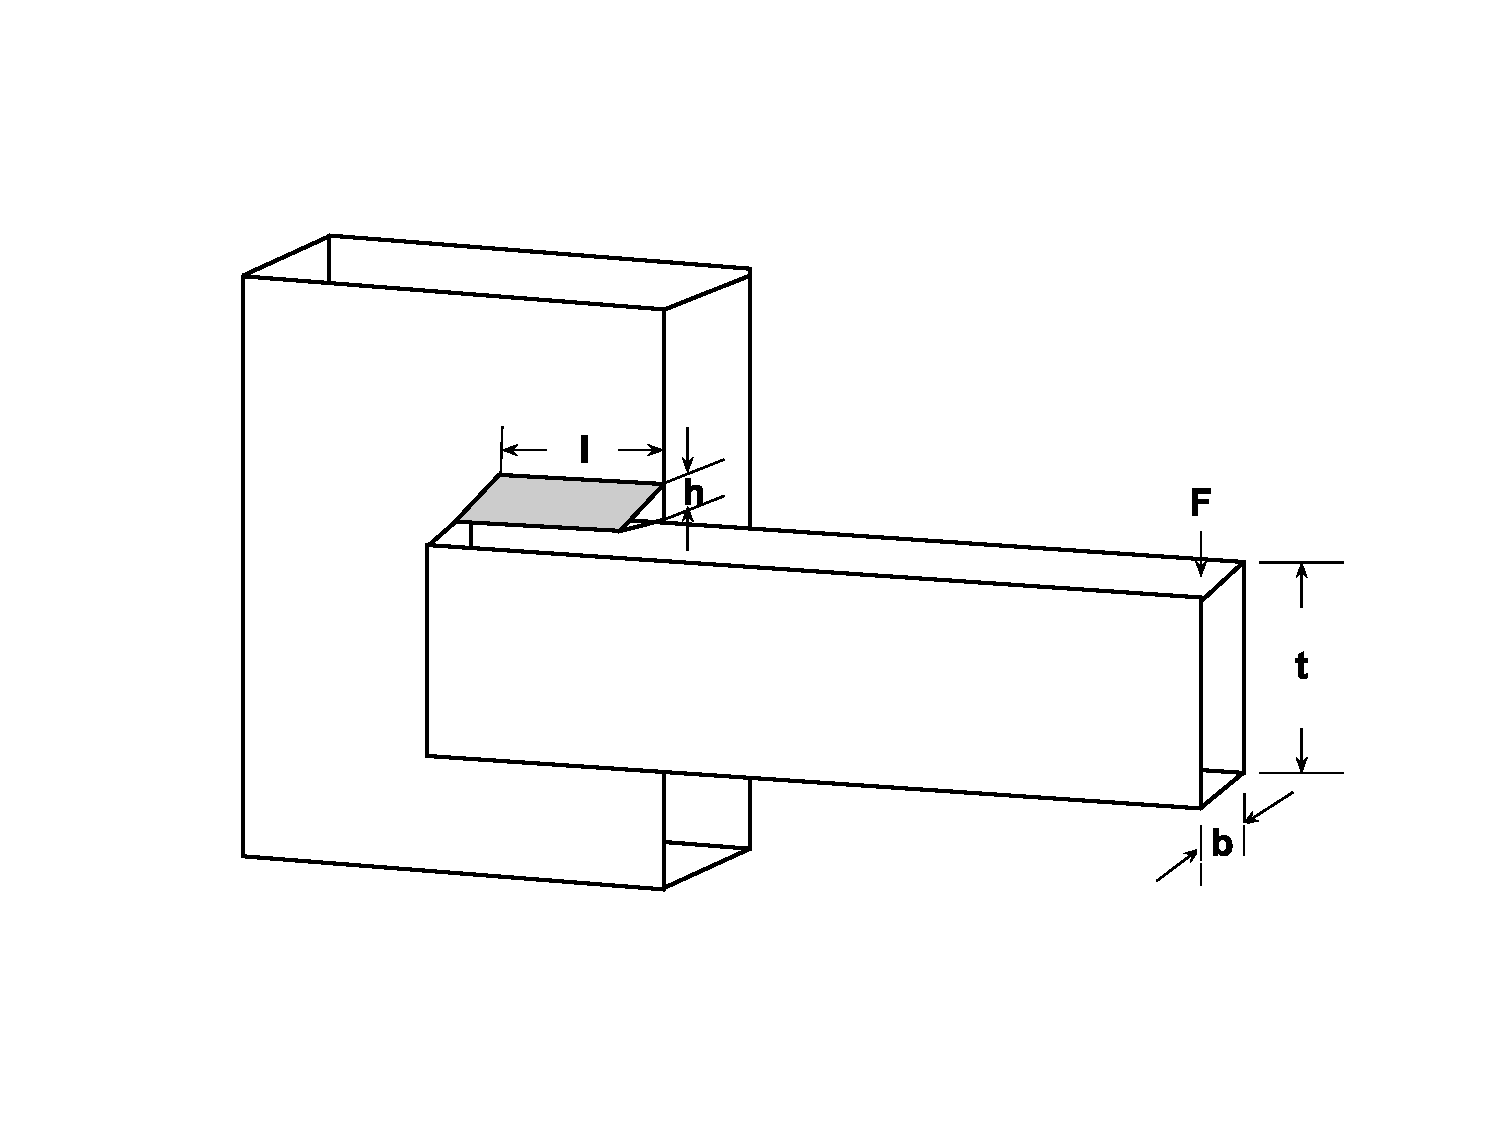
\includegraphics[width=75mm, height=60mm]{dia/wbeam.eps}}
 \caption{Schematics of a welded beam.}
 \label{wbeam}
\end{center}\end{figure}


Welded beam design problem is a well known Multi-objective optimization
problem. Here we adopt the formulation given in \citep{deb10}. The
objective of this problem is to minimize the cost and end deflection of a
beam welded at one end and supporting a load $ F = 6000$ lb at the other.
The overhang portion of the beam has a length of 14 in.There are four
design variables:
\begin{enumerate}
  \item $b \in [0.125, 5] $ thickness of the beam,
  \item $t \in [0.1, 10] $ width of the beam,
  \item $l \in [0.1, 10] $ length of the weld and
  \item $h \in [0.125, 5] $ thickness of the weld.
\end{enumerate}

The complete multi-objective formulation is as follows:

\begin{singlespacing}
  \begin{align}
    \text{Minimize} \quad &f_1(\vec{x}) = C = \left. 1.1047 h ^2 l + 0.04811 t b(14.0 + l) \right. \\
    \text{Minimize} \quad &f_2(\vec{x}) = D = \left. \dfrac{2.1952}{t^3 b} \right. \\
  \text{Subject to:}  & \nonumber \\
  \qquad &g_1(\vec{x}) = \left. 13600 - \tau (\vec{x}) \geqslant 0 \right. ,\\
  \qquad &g_2(\vec{x}) = \left. 30000 - \sigma (\vec{x}) \geqslant 0 \right.,\\
  \qquad &g_3(\vec{x}) = \left. b - h \geqslant 0 \right., \\
  \qquad &g_4(\vec{x}) = \left. P_c(\vec{x}) - 6000 \geqslant 0 \right. 
\end{align}

% \begin{align}
% \end{align}

Where,

\begin{itemize}
  \item $ \tau (\vec{x}) = \sqrt{ \dfrac{(\tau ')^2 + (\tau'')^2 + (l \tau' \tau'')} {\sqrt{ 0.25(l^2 + (h + t)^2)}}}$,
  \item $ \tau' = \dfrac {6000} {\sqrt{2} h l}$,
  \item $ \tau'' = \dfrac { 6000 (14 + 0.5l) \sqrt{0.25(l^2 + (h + t) ^2 )}} { 2 [0.707 h l (\frac{l^2}{12} + 0.25 (h + t) ^2)] } $,
  \item $ \sigma (\vec{x}) = \dfrac {504000} {t^2 b} $,
  \item $P_c (\vec{x}) = 64746.022(1-0.0282346t) t b^3$.
\end{itemize}

\end{singlespacing}    

\section{Analysis of the clutch brake design problem}

Figure \ref{clutch} shows the pareto-front obtained after running local
search on NSGA-II output. NSGA-II was run for 300 generations with a
population size of 5000 and yielded 125 near optimal solutions. The
probability for crossover and mutation were set to 0.79 and 0.5
respectively. Running local search gives a pareto-front consisting of 95
optimal solutions.

\begin{figure}[ht]\begin{center}
 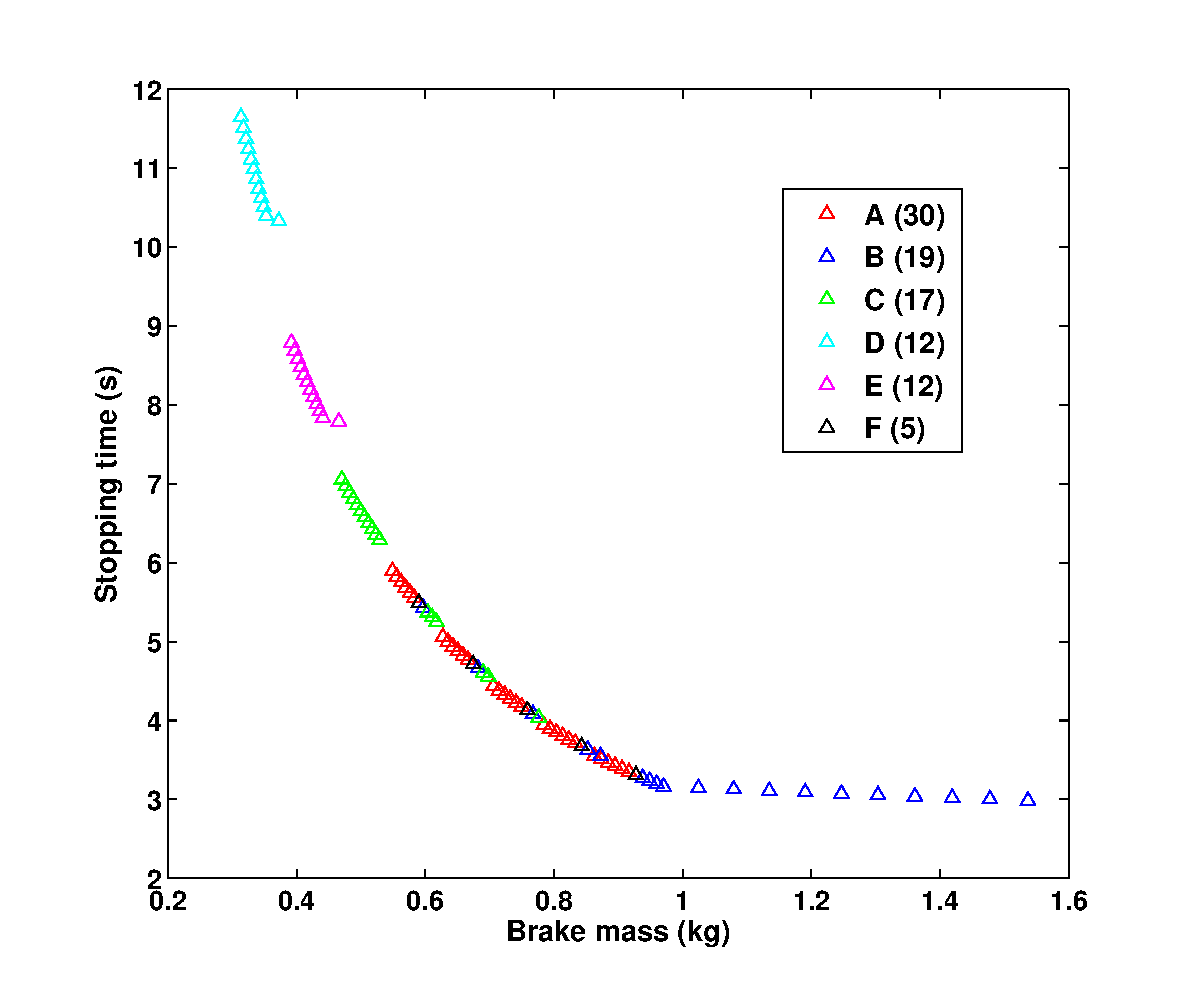
\includegraphics[width=100mm, height=80mm]{dia/clutchParetoClusters.eps}
 \caption{Pareto-front and the clusters of the multiple-disk clutch brake
   design problem. Clusters obtained with $k = 1.9$}
 \label{clutch}
\end{center}\end{figure}


\subsection{Isomap and PCA analysis of the pareto-front} 
Figure \ref{clutchwrv} and \ref{clutchwev} show the results of running
Isomap and PCA on the pareto-front of the clutch brake design problem. The
drop in the residual variance curve for the second Isomap dimension
indicates a manifold dimensionality of one. The PCA explained variance,
however, shows two principal components with significant explained
variances, the first with 80\% explained variance and the second with 17\%.


\begin{figure}[ht]\begin{center}
 \subfloat[Isomap Residual Variance.]{
 \label{clutchwrv} 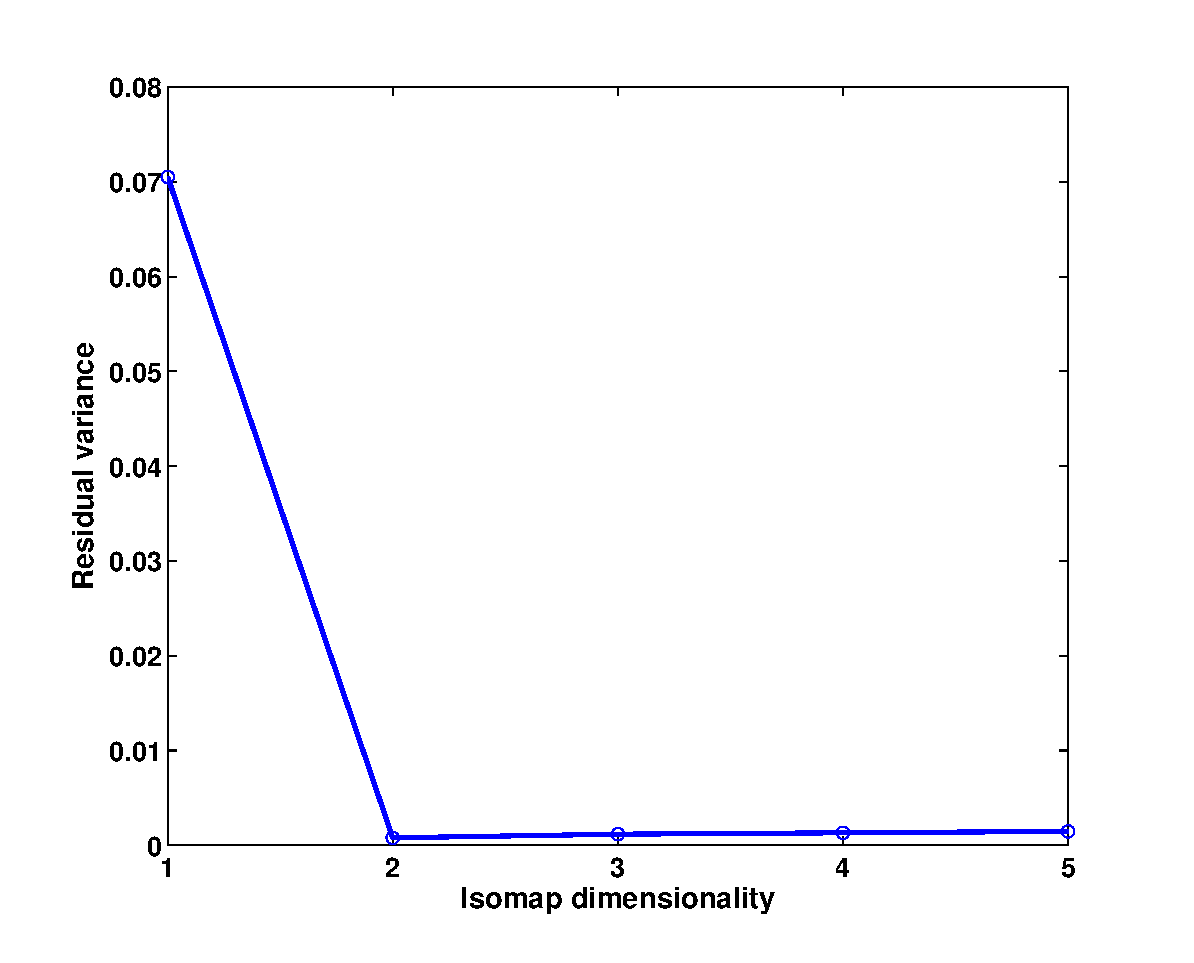
\includegraphics[width=62mm, height=52mm]{dia/clutchRV.eps}}
 \subfloat[PCA Explained variance.]{
 \label{clutchwev} 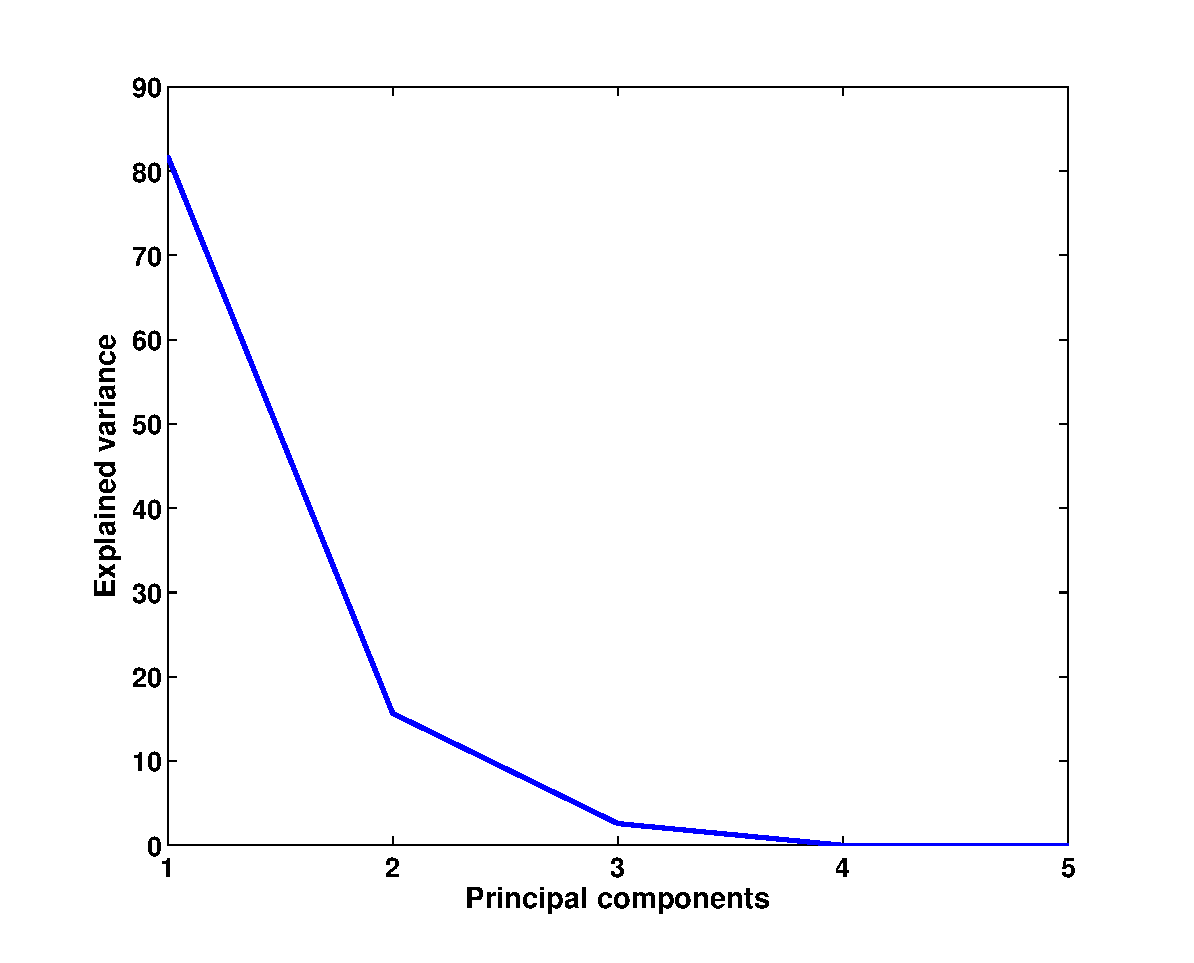
\includegraphics[width=62mm, height=52mm]{dia/clutchEV.eps}}
\caption{Isomap and PCA results for the pareto-front of multiple-disk
  clutch brake problem pareto-front. The manifold dimensionality is one as
  indicated in the Isomap residual variance plot but the PCA explained
  variance shows two significant principal components.}
 \label{clutchWholeVar}
\end{center}\end{figure}

Table \ref{first2clutchPCs} shows the first two significant components of
the pareto-front. Outer radius ($r_o$) has the highest weight in the
first principal component followed by inner radius ($r_i$). The number of
surfaces also has some variation. In the second principal component number
of surfaces ($Z$) is the dominant variable followed by inner radius with a
small weight. The variables thickness ($t$) and actuating force ($F$)
have zero weights in both the significant principal components indicating
they have the same values for all the optimal solutions. The thickness and
actuating force are fixed at the minimum and maximum possible values of 1
and 1000 respectively for all the optimal solutions.


\begin{table}[!ht]
  \centering
  \begin{tabular}{c|c|c|c|c|c|}
    \cline{2-6}
    & $r_{i}$ & $r_{o}$ & $ t $  & $F$ & $Z$ \\
    \hline
    \multicolumn{1}{|c|}{First PC} & 0.578 & 0.806 & 0 & 0 & 0.119\\
    \hline
    \multicolumn{1}{|c|}{Second PC} & -0.207 & 0.004 & 0 & 0 & 0.978\\
    \hline
  \end{tabular}
  \caption{First two principal components of the clutch brake design problem pareto-fron}
  \label{first2clutchPCs}
\end{table}

\subsection{Clustering analysis}
The pareto-front of this problem has a small number (95) of optimal
solutions. The $k$ parameter of the clustering algorithm had to be adjusted
accordingly to obtain a proper distribution of points in clusters. Six
clusters were obtained with $k = 1.9$. The clusters are shown in figure
\ref{clutch}.

Cluster \textbf{A} is the largest cluster with 37 points. It has the
mid-range designs of the clutch brake with stopping times ranging from 3.2
seconds to 6 seconds. Cluster \textbf{B} is composed of the heaviest and
most powerful brake designs, apart from some mid-range designs. It's the
only cluster having designs with weights in excess of 1 kg. Below 1 kg
designs follow a parabolic time vs. weight characteristics, but above 1 kg
designs show a linear relationship, an increase in weight yielding very
little benefit in stopping time. Clusters \textbf{D} and \textbf{E} have
the low end designs with stopping times in excess of 7.5 s. These are the
only clusters that appear as single contiguous chunks in the
pareto-front. Clusters \textbf{A}, \textbf{B}, \textbf{C} and \textbf{E}
have designs in overlapping objective ranges.

Isomap residual variances of the clusters (figure \ref{clutchcrv})
indicate one dimensional manifolds for the clusters, similar to the whole
pareto-front. This verifies the claims of the {\em chunk dimensionality
  conjecture} (section \ref{cdc}). Clusters \textbf{B-C} and \textbf{D-E}
have exactly same residual variances.  Cluster \textbf{A} has the highest
error in reverse mapping the one dimensional Isomap embedding. Clusters
\textbf{D} and \textbf{E} have negligible residual variances. PCA explained
variances for the clusters (figure \ref{clutchcev}) show a single
significant principal component for all the clusters except cluster
\textbf{A}.


\begin{figure}[ht]\begin{center}
 \subfloat[Isomap Residual Variance.]{
 \label{clutchcrv} 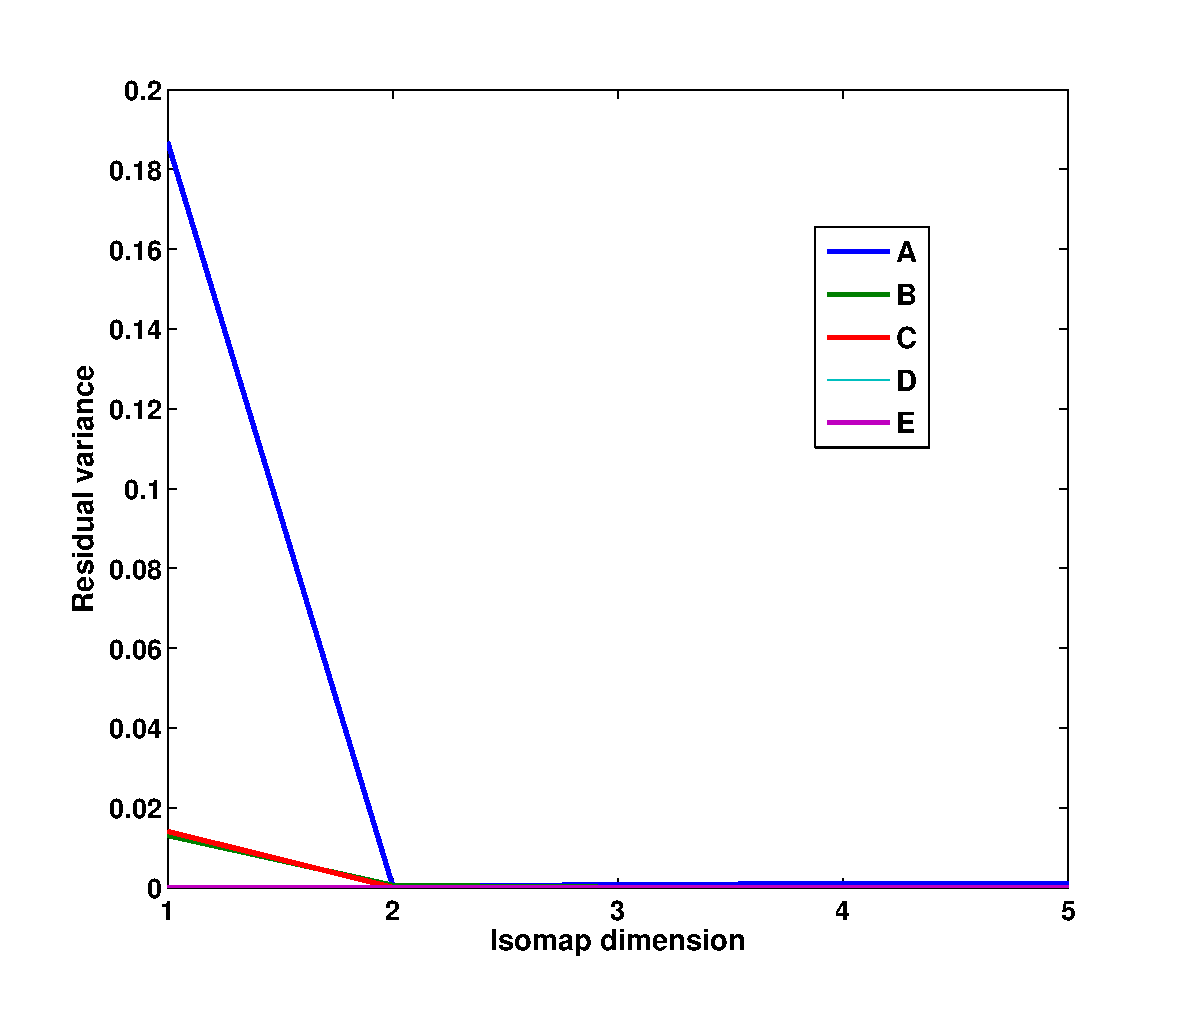
\includegraphics[width=62mm, height=52mm]{dia/clutchClustersRV.eps}}
 \subfloat[PCA Explained variance.]{
 \label{clutchcev} 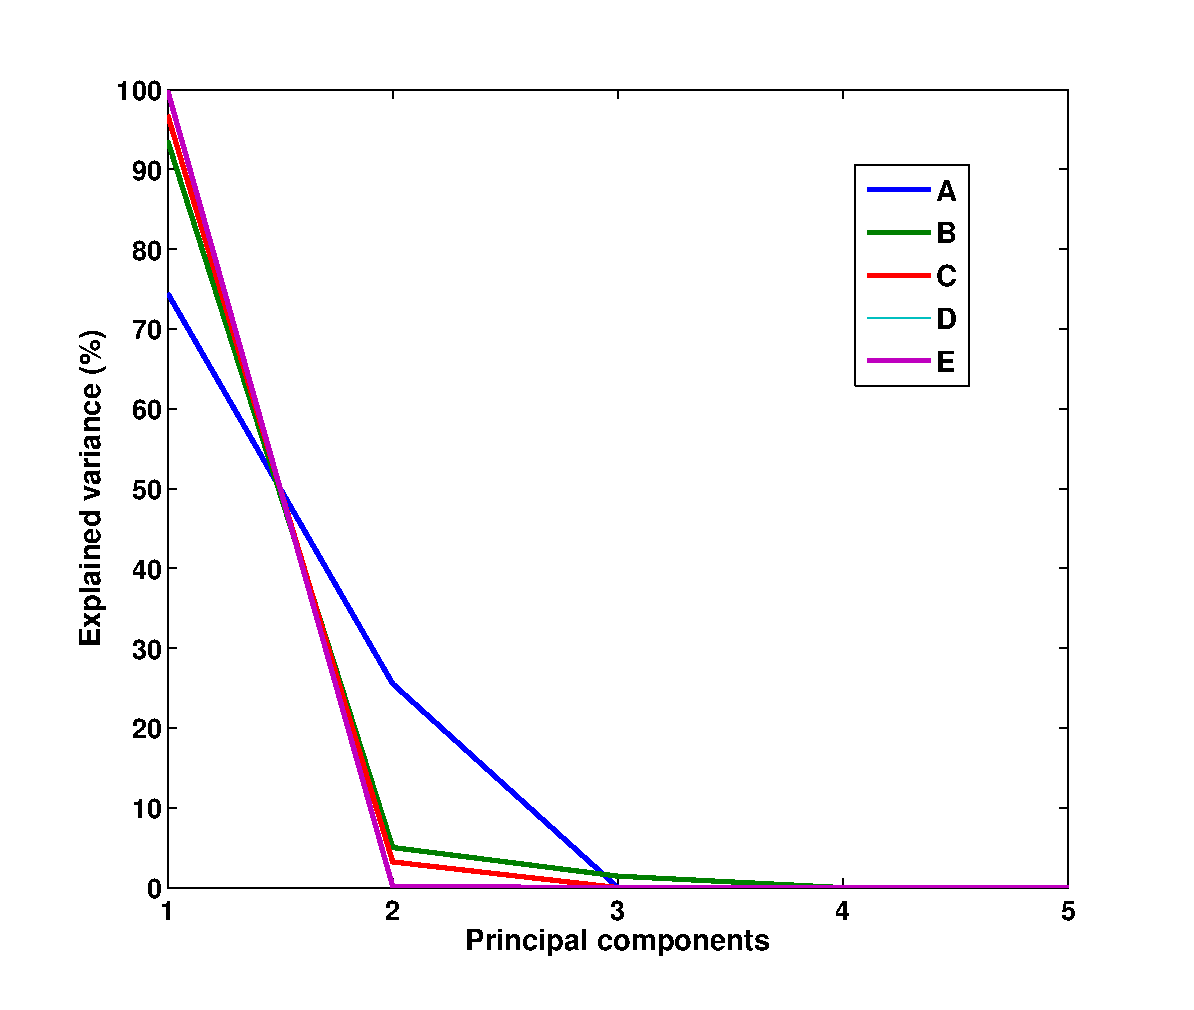
\includegraphics[width=62mm, height=52mm]{dia/clutchClustersEV.eps}}
\caption{Isomap and PCA results for the clusters of multiple-disk clutch
  brake problem. The manifold dimensionality of all the clusters is one,
  though cluster \textbf{A} has linear dimensionality of two indicated by
  two significant principal components in its explained variance plot.}
 \label{clutchClustersVar}
\end{center}\end{figure}


\begin{table}[!ht]
  \centering
  \begin{tabular}{c|c|c|c|c|c|}
    \cline{2-6}
    & $r_{i}$ & $r_{o}$ & $ t $  & $F$ & $Z$ \\
    \hline
    \multicolumn{1}{|c|}{\multirow{2}{*}{\textbf{A}}} & 0.707 & 0.707 & 0 & 0 & 0\\ \cline{2-6}
    \multicolumn{1}{|c|}{}& 0 & 0 & 0 & 0 & 1\\
    \hline
    \multicolumn{1}{|c|}{\textbf{B}} & 0.236 & 0.960 & 0 & 0 & 0.146\\
    \hline
    \multicolumn{1}{|c|}{\textbf{C}} & 0.703 & 0.703 & 0 & 0 & 0.097\\
    \hline
    \multicolumn{1}{|c|}{\textbf{D}} & 0.694 & 0.719 & 0 & 0 & 0\\
    \hline
    \multicolumn{1}{|c|}{\textbf{E}} & 0.694 & 0.719 & 0 & 0 & 0\\
    \hline
    \multicolumn{1}{|c|}{\textbf{F}} & 0 & 0 & 0 & 0 & 1\\
    \hline
  \end{tabular}
  \caption{Significant principal components of the clutch brake design problem clusters. $t$ and $F$ have no weights in any principal component. The inner and outer radii($r_i$ and $r_o$) show the highest variation for each cluster. The second component is parallel to the {\em number of friction surfaces (Z)} dimension.}
  \label{first2clutchPCs}
\end{table}

Table \ref{first2clutchPCs} shows the principal components of the
clusters. For most of the clusters, the radius variables have similar
weights. In cluster \textbf{B} the outer radius has higher weight than the
inner radius.  The second principal component of cluster \textbf{A} has
entirely composed of a single variable $Z$ only. Clusters \textbf{D} and
\textbf{E} have exactly the same components. The cluster \textbf{F} has 
variable $Z$ as its single Principal component.

\subsection{Discussion}

The most important fact that comes out of this analysis is that all optimal
clutch brakes should be designed with disks with smallest possible
thickness.  Secondly, a clutch brake must be designed for maximum actuating
force only, since the stopping time is inversely proportional to the
actuating force. The stopping time is also dependent on the friction area
as is evident from the figure \ref{clutchrVsZ}. A higher outer radius and a
larger number of friction surfaces (no. of disks) allow for a larger
contact area, but increasing the number of disks also increases the weight
of the design.  This trade-off is visible in all the clusters. The fact
that radius variables show greater variation across all clusters suggests
that to reduce the stopping time increasing the radial dimension is the
more economical option.


\begin{figure}[ht]\begin{center}
 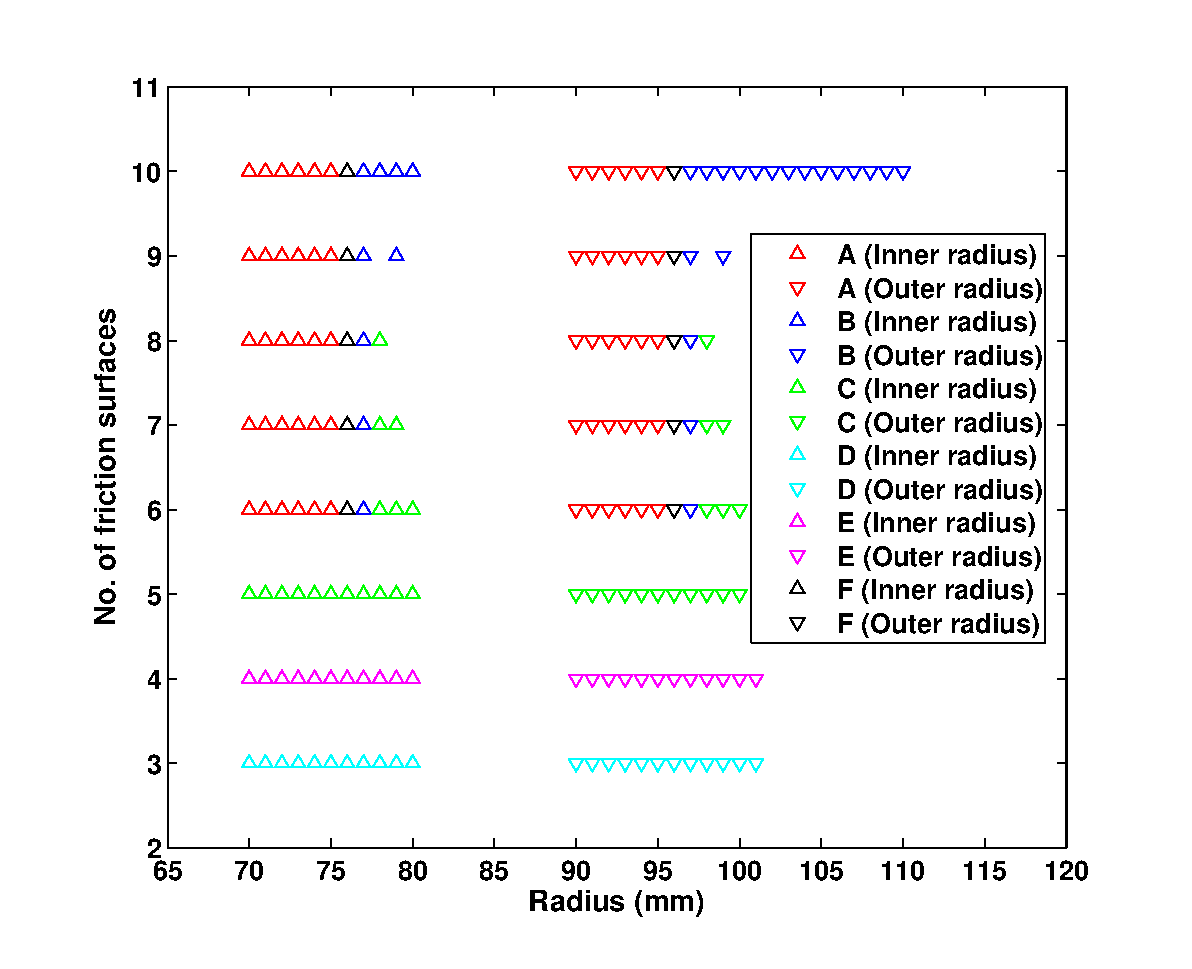
\includegraphics[width=100mm, height=80mm]{dia/clutchrVsZ.eps}
 \caption{Radius Vs. no. of friction surface plot for pareto-front
   clusters. Clusters \textbf{A}, \textbf{B}, \textbf{C} and \textbf{F} are
   distributed in four lines each while \textbf{D}, \textbf{E} and
   \textbf{F} are composed of single lines.}
 \label{clutchrVsZ}
\end{center}\end{figure}

The two dimensional nature of cluster \textbf{A} can be explained by this
plot. \textbf{A} has designs with small variation in radial dimensions
except in very heavy clutch brakes, those occupying the linear region in
plot \ref{clutch}. For the linear region designs, the number of disks is
maximum and the only way to design more powerful brakes is by increasing
the outer radius to increase the friction area. If the clustering had been
done in the design variables space only we would have clusters on the basis
of the number of contact surfaces only. Clustering in the combined
objective-decision variable space gives more meaningful clusters, which
have functionally similar designs.





\section{Analysis of welded beam design problem}
The NSGA-II run for the welded beam design problem yielded 500 solutions
with a population size of 500 running for 200 hundred generations. The
crossover and mutation probability were set to 0.73 and 0.53. After local
search the pareto-front obtained had 491 optimal solutions.  Figure
\ref{wbeam} shows the final pareto-front.


\begin{figure}[ht]\begin{center}
 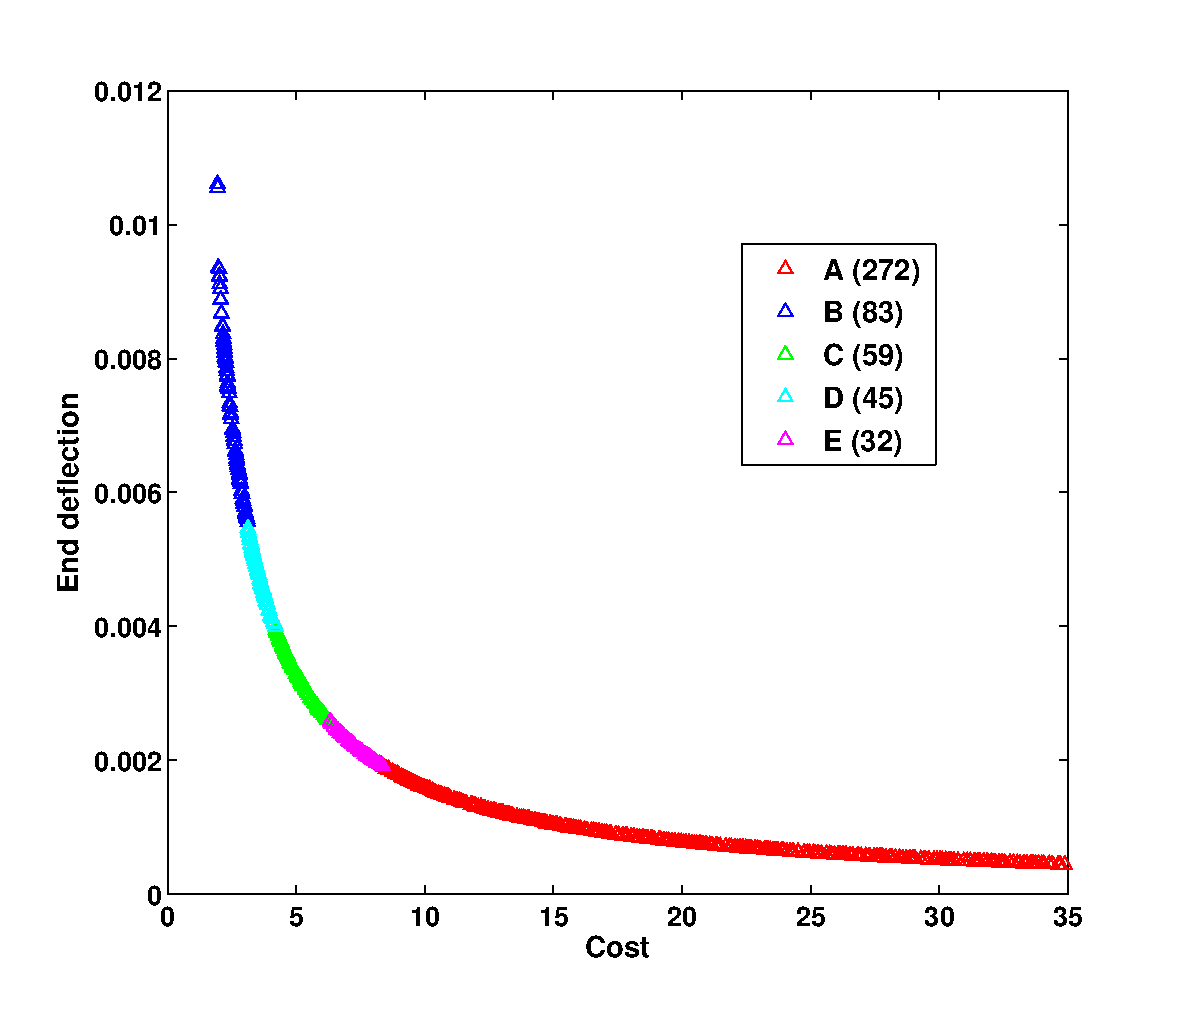
\includegraphics[width=100mm, height=80mm]{dia/wbeamParetoClusters.eps}
 \caption{Pareto-front and clusters of the welded beam design
   problem. Obtained with $k = 2$. The clusters in the extremes are the
   largest while those around the knee of the curve are relatively smaller}
 \label{wbeam}
\end{center}\end{figure}

\section{Isomap and PCA analysis of the pareto-front}

The residual variance plot shown in figure \ref{wbeamwrv} shows the largest
drop for dimension 2. Their is some further drop going from second two
third dimensional embedding. This indicates a manifold dimensionality of
one. The PCA explained variance (figure \ref{wbeamwev}) also shows only one
significant principal component with an explained variance of 93\%. Table
\ref{firstWbeamPC} shows the first principal component of the pareto-front.
The beam thickness ($b$) is the design variable with the highest weight in
the principal component. Weld thickness ($h$) and length of the weld ($l$)
have similar weights, albeit that of $l$ being in the reverse direction.
Width of the beam ($t$) is the least varying variable of all.

\begin{figure}[ht]\begin{center}
 \subfloat[Isomap Residual Variance for welded beam problem pareto-front]{
 \label{wbeamwrv} 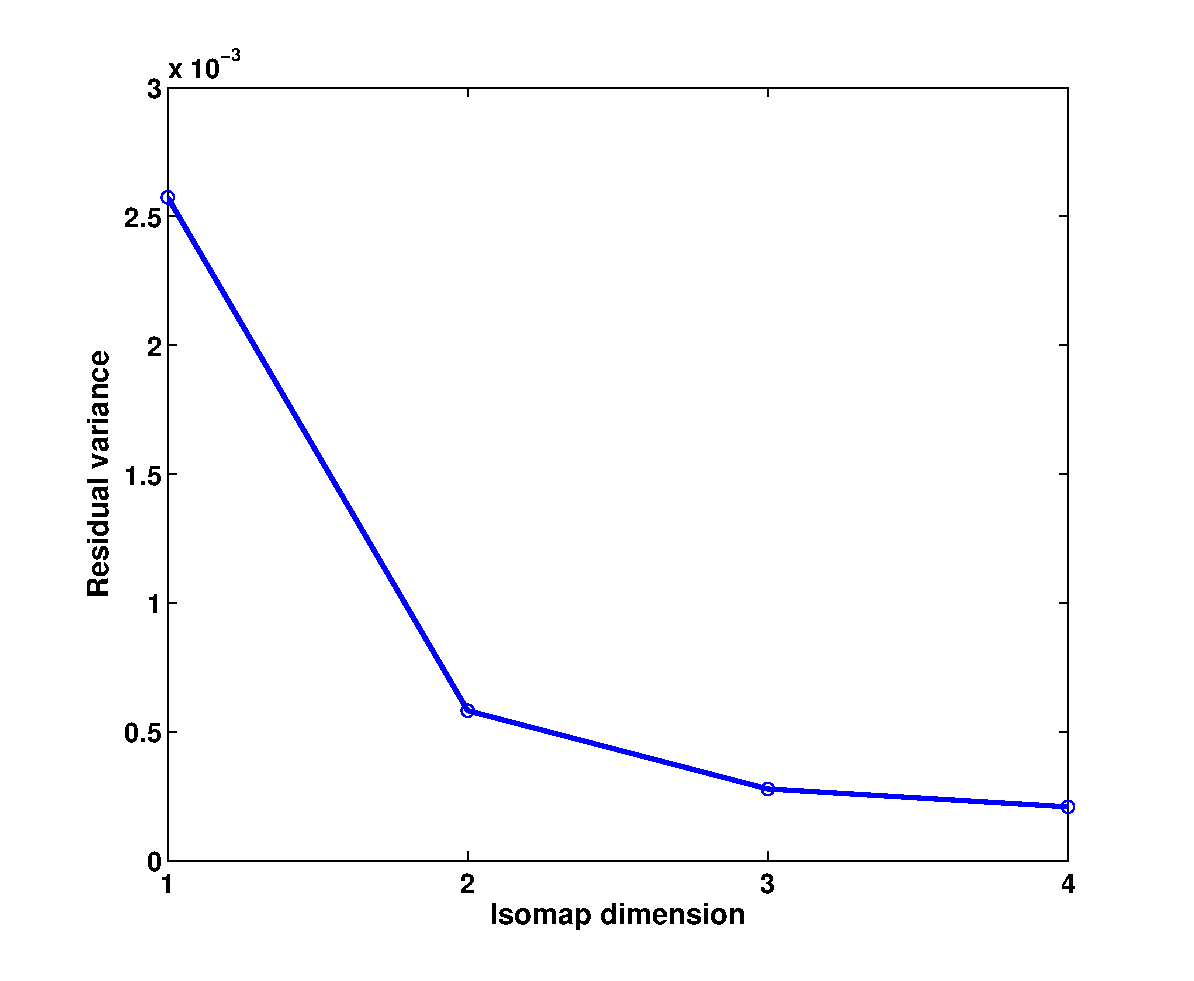
\includegraphics[width=62mm, height=52mm]{dia/wbeamWholeRV.eps}}
 \subfloat[PCA Explained variance for pareto-front of welded beam problem]{
 \label{wbeamwev} 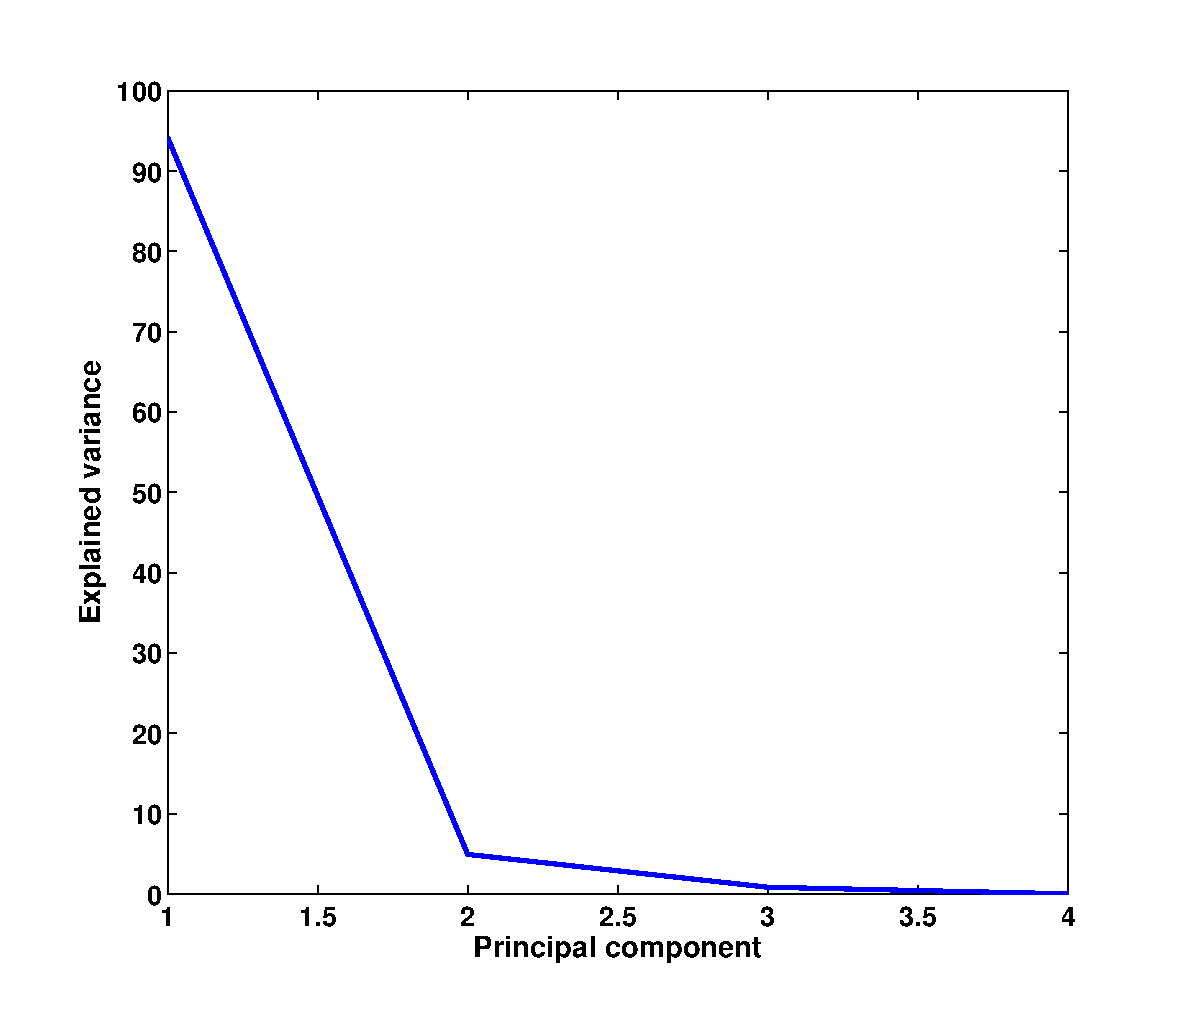
\includegraphics[width=62mm, height=52mm]{dia/wbeamWholeEV.eps}}
 \caption{Isomap and PCA results for the welded beam design problem}
 \label{wbeamWholeVar}
\end{center}\end{figure}


\begin{table}[!ht]
  \centering
  \begin{tabular}{c|c|c|c|c|}
    \cline{2-5}    
    & $b$ & $t$ & $l$  & $h$ \\
    \hline
    \multicolumn{1}{|c|}{First PC} & 0.903 & 0.001 & -0.278 & 0.325\\
    \hline
  \end{tabular}
  \caption{First two principal components of the clutch brake design problem pareto-front}
  \label{firstWbeamPC}
\end{table}


\subsection{Clustering analysis}
A large number of specific clusters could be obtained by suitably setting
the parameters of the algorithm, but we analyze only 5 clusters for the
sake of simplicity. The clusters are shown in figure \ref{wbeam}.

Clusters \textbf{A} and \textbf{B} have the largest number of optimal
solutions. They occupy the linear extremes of the pareto-front curve. Three
clusters are concentrated around the knee of the curve. Cluster \textbf{A}
has the costliest and sturdiest designs, while cluster \textbf{B} has the
cheapest and the weakest beams. Clusters \textbf{C}, \textbf{D} and
\textbf{E} have beams with mid range end deflection and cost.


\begin{figure}[ht]\begin{center}
 \subfloat[Isomap Residual Variances.]{
 \label{wbeamcrv} 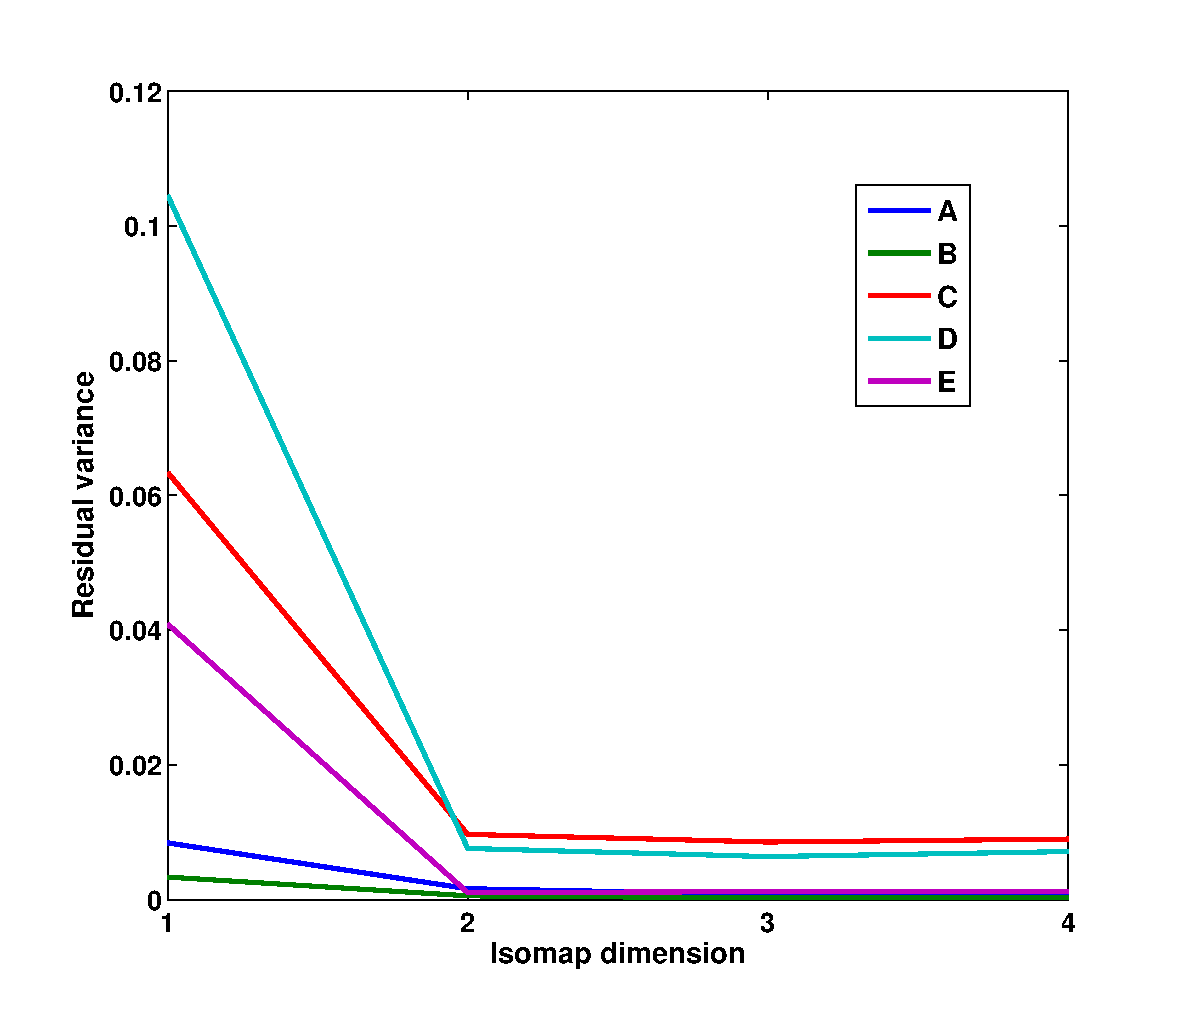
\includegraphics[width=62mm, height=52mm]{dia/wbeamClustersRV.eps}}
 \subfloat[PCA Explained variances.]{
 \label{wbeamcev} 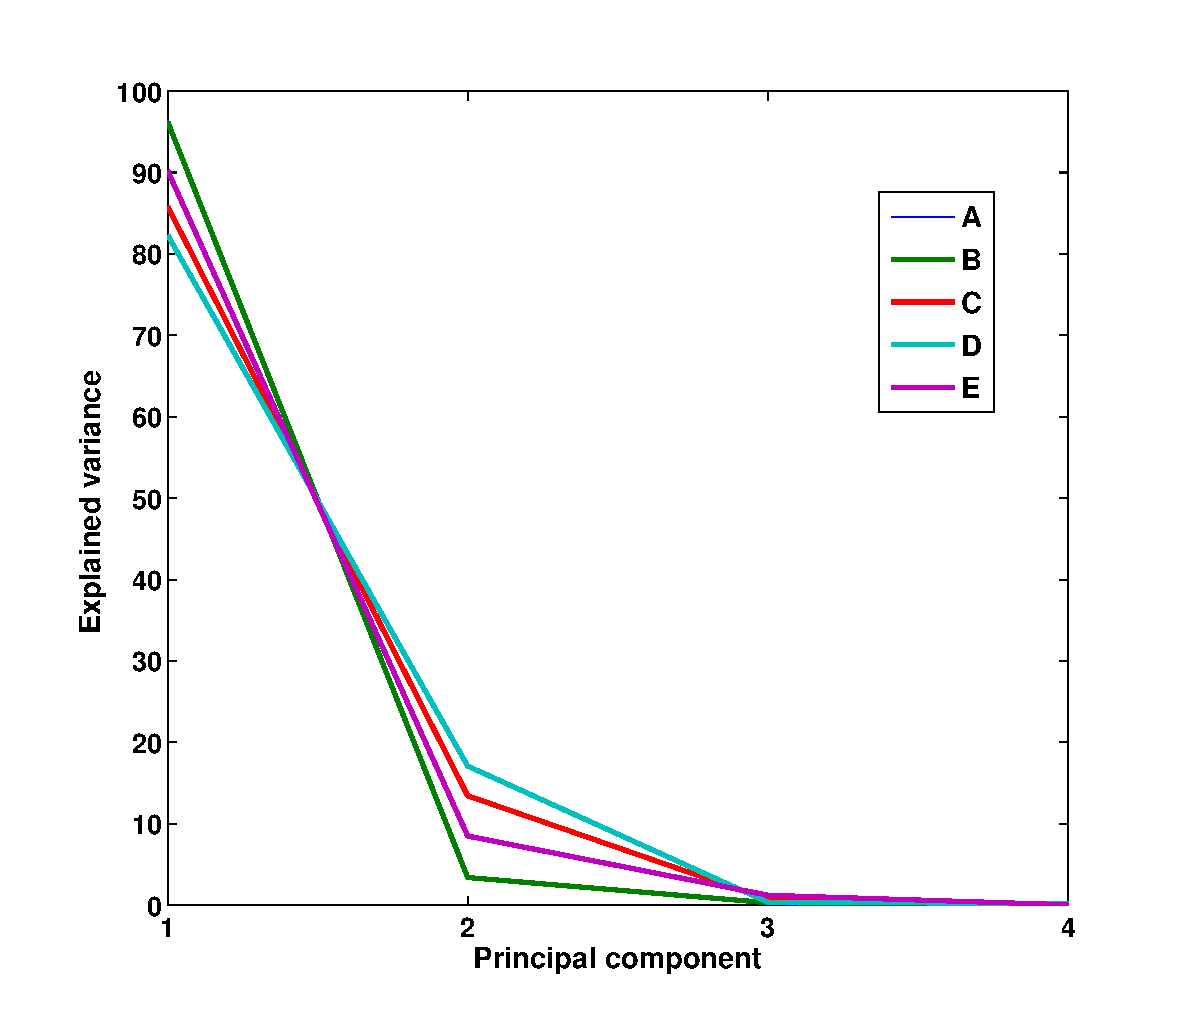
\includegraphics[width=62mm, height=52mm]{dia/wbeamClustersEV.eps}}
\caption{Isomap and PCA results for the clusters of welded beam design
  problem. All the clusters are one dimensional manifolds but clusters
  \textbf{C} and \textbf{D} have two linear dimensions as they have two
  significant components.}
 \label{wbeamClustersVar}
\end{center}\end{figure}

The Iosmap residual variances for all the clusters suggest one dimensional
manifolds clusters as all the curves have the largest drop for second
dimension. Clusters \textbf{D} and \textbf{C} have relatively higher
residual variances than other clusters. The PCA explained variance for
these clusters also show two significant components. The explained variance
plots for clusters \textbf{A} and \textbf{B} are almost the same resulting
in overlapping lines in the plot. The cluster E also has two significant
components.

Thickness of the beam ($b$) is the predominant variable in the principal
component of the cluster \textbf{A} (table \ref{first2wbeamPCs}) while
length of the weld ($l$) is the predominant variable in cluster
\textbf{B}. These two are at the two extremes of the pareto-front, the
former having designs with least deflection and highest cost and the latter
having cheapest designs with large end deflections. The clusters around the
knee of the pareto-front curve also have their two significant components
in the $b$ - $l$ plane with first component leaning more towards the $l$
direction and second component leaning towards $b$. For all the clusters
width of the beam ($t$) has the least variation. For all the optimal
designs, the width of the beam is approximately maximum possible value of
10.

% b - thickness of the beam
% t - width of the beam
% l - length of the weld
% h - thickness of the weld




\begin{table}[!ht]
  \centering
  \begin{tabular}{c|c|c|c|c|}
    \cline{2-5}
    & $b$ & $t$ & $ l$  & $h$ \\
    \hline
    \multicolumn{1}{|c|}{\textbf{A}} & 0.965 & 0 & -0.06 & 0.249 \\
    \hline
    \multicolumn{1}{|c|}{\textbf{B}} & 0.126 & 0.068 & -0.982 & 0.115\\
    \hline
    \multicolumn{1}{|c|}{\multirow{2}{*}{\textbf{C}}} & 0.435 & 0 & -0.755 & 0.488 \\ \cline{2-5}
    \multicolumn{1}{|c|}{}& 0.897 & 0.006 & 0.404 & -0.174\\
    \hline
    \multicolumn{1}{|c|}{\multirow{2}{*}{\textbf{D}}} & 0.309 & 0 & -0.883 & 0.351 \\ \cline{2-5}
    \multicolumn{1}{|c|}{}& 0.949 & 0.011 & 0.307 & -0.06\\
    \hline
    \multicolumn{1}{|c|}{\multirow{2}{*}{\textbf{E}}} & 0.381 & 0.002 & -0.616 & 0.688 \\ \cline{2-5}
    \multicolumn{1}{|c|}{}& 0.924 & 0.019 & 0.256 & -0.282\\
    \hline
  \end{tabular}
  \caption{Significant principal components of the pareto-front clusters of the welded beam design problem. The one dimensional clusters have $b$ and $l$ as the predominant variables. Two dimensional clusters also have their significant components in the $b$-$l$ plane. $t$ is the least varying variable in all the clusters.}
  \label{first2wbeamPCs}
\end{table}

\subsection{Discussion}
Width of the beam ($t$) variable has the least variation for all the
clusters. All the optimal designs use the maximum possible value of the
width beam. This suggests that a welded beam should be as wide as possible,
other design variables should be adjusted to obtain suitable designs. In
cluster \textbf{A} of the sturdiest designs, designs tend to vary in the
thickness of the beam the most with other variables limited to small ranges
of variation. The maximum value of $l$ an $h$ are 1.39 and 2.49 which are
significantly less than their maximum possible of 10 and 5
respectively. This suggests that increasing the size of the weld in $l$ and
$h$ beyond certain limit doesn't help in improving the sturdiness much,
though increasing thickness of the beam may improve the end deflection. In
cluster \textbf{B} the cost is minimum though the designs have larger end
deflection than in other clusters. In this cluster, $l$ is the variable
that varies the most, with other variables showing less variation. $l$ is
increased or decreased to increase or decrease the cost.

% b - thickness of the beam
% t - width of the beam
% l - length of the weld
% h - thickness of the weld







 